% =============================================================================
% SECCION: LA PARADOJA DEL DIRECTIONAL ACCURACY
% =============================================================================

\section{La Paradoja del Directional Accuracy}
\label{sec:da_paradox}

Un hallazgo contraintuitivo de este estudio es que el Directional Accuracy (DA)---la m\'etrica m\'as com\'unmente utilizada para evaluar modelos de predicci\'on de direcci\'on de mercado---no es un predictor confiable de rentabilidad en estrategias de trading.

\subsection{El Hallazgo Contraintuitivo}
\label{subsec:counterintuitive}

\subsubsection{Intuici\'on Na\"ive vs Realidad}

La intuici\'on convencional sugiere que un modelo que predice correctamente la direcci\'on del mercado con mayor frecuencia deber\'ia generar mayores retornos. Sin embargo, nuestros resultados emp\'iricos contradicen esta suposici\'on:

\begin{equation}
\rho(\text{DA}, \text{Return}) = -0.14
\end{equation}

La correlaci\'on entre Directional Accuracy y retorno total es \textbf{ligeramente negativa}, indicando que modelos con mayor DA no necesariamente generan mejores retornos.

\subsubsection{Evidencia Emp\'irica}

\begin{table}[htbp]
\centering
\caption{Paradoja DA vs Retorno: Casos Ilustrativos}
\label{tab:da_paradox}
\begin{tabular}{@{}lrrr@{}}
\toprule
\textbf{Modelo} & \textbf{DA General} & \textbf{Retorno Total} & \textbf{Categor\'ia} \\
\midrule
GARCH & 54.3\% & -6.2\% & Alto DA, Retorno Negativo \\
Theta & 54.6\% & -19.2\% & Alto DA, Retorno Negativo \\
ExponentialSmoothing & 53.8\% & -4.6\% & Alto DA, Retorno Negativo \\
\midrule
Ridge & 52.7\% & +318.8\% & DA Medio, Mejor Retorno \\
CNN\_LSTM & 50.8\% & +207.1\% & DA Bajo, Alto Retorno \\
GradientBoosting & 51.2\% & +267.5\% & DA Medio, Alto Retorno \\
\bottomrule
\end{tabular}

\vspace{0.2cm}
\small\textit{Nota: DA calculado como porcentaje de d\'ias donde la predicci\'on de direcci\'on coincide con el movimiento realizado del mercado.}
\end{table}

\begin{figure}[htbp]
\centering
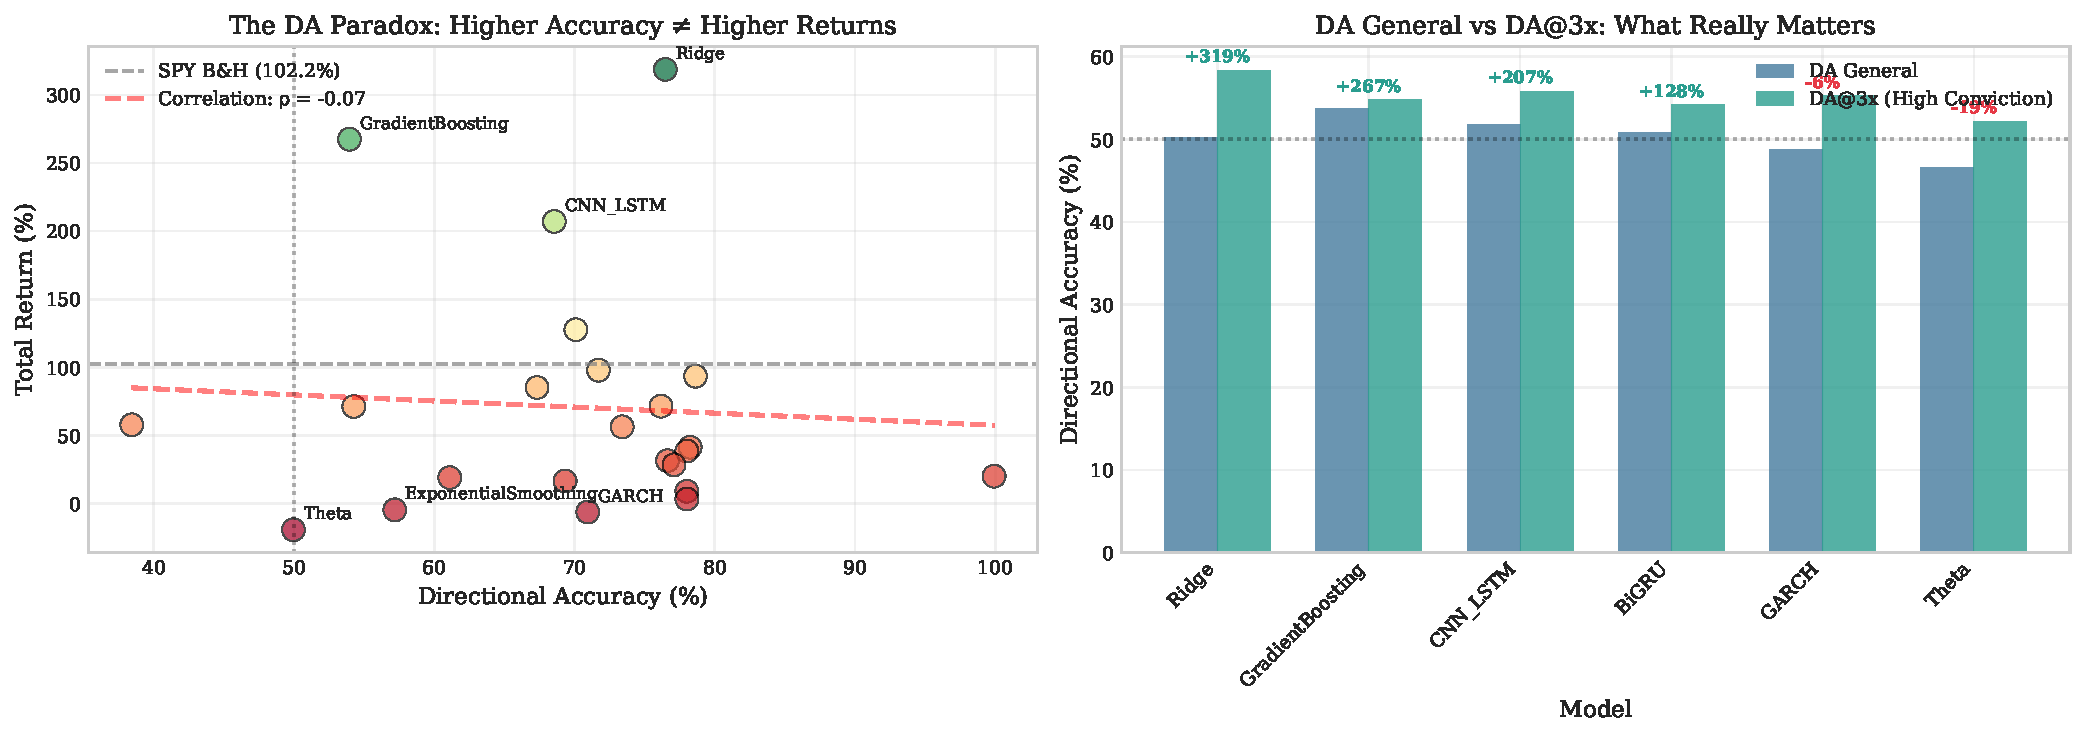
\includegraphics[width=\textwidth]{figures/da_vs_return_paradox.pdf}
\caption{La Paradoja del Directional Accuracy. Panel izquierdo: Scatter plot de DA vs Retorno Total mostrando correlaci\'on negativa ($\rho = -0.14$). Panel derecho: Comparaci\'on de DA General vs DA@3x (hit rate en posiciones apalancadas) para modelos seleccionados. Los retornos se indican sobre cada par de barras.}
\label{fig:da_paradox}
\end{figure}

\subsection{Explicaci\'on de la Paradoja}
\label{subsec:paradox_explanation}

\subsubsection{El DA Trata Todos los D\'ias como Iguales}

El Directional Accuracy asigna el mismo peso a cada predicci\'on, independientemente de:
\begin{itemize}
    \item La magnitud del movimiento del mercado
    \item La posici\'on que tom\'o el modelo
    \item El momento del ciclo de mercado
\end{itemize}

\textbf{Ejemplo ilustrativo:}
\begin{verbatim}
D\'ia 1: Mercado +0.1% | Modelo predice correctamente | +
D\'ia 2: Mercado +0.1% | Modelo predice correctamente | +
D\'ia 3: Mercado -3.0% | Modelo falla               | -

DA = 66.7% (2/3 aciertos)
Pero P&L = NEGATIVO (la p\'erdida del d\'ia 3 supera las ganancias)
\end{verbatim}

\subsubsection{Lo Que Realmente Importa: Asimetr\'ia Condicional}

La rentabilidad de una estrategia de trading depende de tres factores que el DA no captura:

\begin{enumerate}
    \item \textbf{Cu\'ando aciertas}: Acertar en d\'ias de movimientos grandes importa m\'as que acertar en d\'ias tranquilos.

    \item \textbf{Cu\'anto apuestas}: El tama\~no de la posici\'on cuando aciertas vs cuando fallas determina el P\&L.

    \item \textbf{Asimetr\'ia ganancia/p\'erdida}: El ratio entre ganancia promedio y p\'erdida promedio (Profit Factor).
\end{enumerate}

\subsection{El Indicador DA@3x: Una M\'etrica M\'as Relevante}
\label{subsec:da_3x}

Proponemos el indicador \textbf{DA@3x} (Directional Accuracy en posiciones apalancadas) como una m\'etrica m\'as predictiva de rentabilidad:

\begin{equation}
\text{DA@3x} = \frac{\sum_{t: \text{pos}_t = 3} \mathbf{1}[r_t^{mkt} > 0]}{\sum_{t} \mathbf{1}[\text{pos}_t = 3]}
\end{equation}

donde $\mathbf{1}[\cdot]$ es la funci\'on indicadora.

\subsubsection{Comparaci\'on DA vs DA@3x}

\begin{table}[htbp]
\centering
\caption{DA General vs DA@3x: El Predictor de Rentabilidad}
\label{tab:da_vs_da3x}
\begin{tabular}{@{}lrrrr@{}}
\toprule
\textbf{Modelo} & \textbf{DA General} & \textbf{DA@3x} & \textbf{\% Tiempo 3x} & \textbf{Retorno} \\
\midrule
Ridge & 52.7\% & 58.3\% & 29.5\% & +318.8\% \\
GradientBoosting & 51.2\% & 56.8\% & 84.6\% & +267.5\% \\
CNN\_LSTM & 50.8\% & 55.8\% & 33.2\% & +207.1\% \\
BiGRU & 52.1\% & 54.9\% & 28.7\% & +127.7\% \\
\midrule
GARCH & 54.3\% & 55.2\% & 25.8\% & -6.2\% \\
Theta & 54.6\% & 52.1\% & 15.3\% & -19.2\% \\
\bottomrule
\end{tabular}

\vspace{0.2cm}
\small\textit{Nota: DA@3x = hit rate cuando el modelo est\'a en posici\'on 3x (UPRO). \% Tiempo 3x indica qu\'e fracci\'on del per\'iodo el modelo estuvo en posici\'on apalancada.}
\end{table}

\subsubsection{Interpretaci\'on}

Los modelos rentables se distinguen por:

\begin{enumerate}
    \item \textbf{Mayor DA@3x que DA general}: Ridge tiene 52.7\% DA general pero 58.3\% DA@3x---acierta m\'as cuando apuesta fuerte.

    \item \textbf{Selectividad en el apalancamiento}: Ridge solo usa posici\'on 3x el 29.5\% del tiempo, reserv\'andola para se\~nales de alta confianza.

    \item \textbf{Protecci\'on en incertidumbre}: Cuando no tiene confianza, permanece en cash (62\% del tiempo para Ridge).
\end{enumerate}

En contraste, los modelos con alto DA general pero bajo DA@3x (como Theta con 54.6\% vs 52.1\%) tienden a ``acertar en los d\'ias que no importan''.

\subsection{Implicaciones para el Dise\~no de Estrategias}
\label{subsec:strategy_implications}

\subsubsection{No Optimizar por DA}

Este hallazgo tiene implicaciones importantes para el dise\~no de estrategias de trading:

\begin{tcolorbox}[colback=gray!5!white,colframe=gray!75!black,title=Implicaci\'on Clave]
Optimizar un modelo para maximizar Directional Accuracy puede ser contraproducente. En su lugar, se debe optimizar por m\'etricas que capturen la asimetr\'ia entre ganancias y p\'erdidas condicionales al tama\~no de la posici\'on.
\end{tcolorbox}

\subsubsection{M\'etricas Alternativas Recomendadas}

En lugar de DA, recomendamos evaluar modelos de trading usando:

\begin{enumerate}
    \item \textbf{Sharpe Ratio}: Captura el trade-off riesgo-retorno
    \item \textbf{Profit Factor}: Ratio entre ganancia promedio y p\'erdida promedio por trade
    \item \textbf{DA@3x}: Hit rate en posiciones de alta convicci\'on
    \item \textbf{Retorno Neto}: La m\'etrica final que realmente importa
\end{enumerate}

\subsubsection{El Valor de la Selectividad}

El \'exito del modelo Ridge ilustra el valor de la selectividad:

\begin{itemize}
    \item \textbf{No predice mejor en general}: DA = 52.7\%, apenas sobre el azar
    \item \textbf{Sabe cu\'ando apostar fuerte}: DA@3x = 58.3\%, significativamente mejor
    \item \textbf{Sabe cu\'ando no apostar}: 62\% del tiempo en cash
    \item \textbf{Resultado}: +318.8\% de retorno, el mejor de todos los modelos
\end{itemize}

\subsection{Conexi\'on con la Literatura}
\label{subsec:literature_connection}

Este hallazgo es consistente con la literatura sobre trading y gesti\'on de portafolios:

\textbf{\citet{lopezdeprado2018}} argumenta que las m\'etricas tradicionales de evaluaci\'on de modelos predictivos (como $R^2$ o accuracy) son inadecuadas para evaluar estrategias de trading, donde lo que importa es la rentabilidad ajustada por riesgo.

\textbf{La paradoja de Grossman-Stiglitz} \citep{grossman1980} sugiere que en mercados eficientes, la capacidad predictiva marginal (como un DA ligeramente superior al 50\%) puede ser suficiente para generar alfa si se combina con una estrategia de posicionamiento inteligente.

\textbf{El criterio de Kelly} \citep{kelly1956} formaliza la idea de que el tama\~no \'optimo de la apuesta depende no solo de la probabilidad de ganar, sino tambi\'en de las magnitudes de ganancia y p\'erdida---exactamente lo que el DA no captura.

\subsection{Resumen de la Secci\'on}
\label{subsec:da_summary}

\begin{tcolorbox}[colback=blue!5!white,colframe=blue!75!black,title=Resumen: La Paradoja del DA]
\begin{enumerate}
    \item El Directional Accuracy (DA) no es un predictor confiable de rentabilidad ($\rho = -0.14$)
    \item Modelos con DA $>$ 54\% generaron retornos negativos
    \item Modelos con DA $\approx$ 51-52\% generaron los mejores retornos
    \item El indicador DA@3x (hit rate en posiciones apalancadas) es m\'as predictivo
    \item Los modelos rentables se caracterizan por \textbf{selectividad}, no por \textbf{frecuencia} de aciertos
    \item Implicaci\'on: Optimizar por DA puede ser contraproducente para estrategias de trading
\end{enumerate}
\end{tcolorbox}

